\chapter{KẾT QUẢ VÀ THẢO LUẬN}\label{chap3_intro}
\vspace{-40pt}

 
\section{SẢN PHẨM/KẾT QUẢ ĐẠT ĐƯỢC}
\subsection{Kết quả 1}
Nội dung văn bản 

Nội dung đoạn 1


Nội dung đoạn 2 nếu có

\subsection{Kết quả 2}


\subsection{Kết quả 3}


\section{THẢO LUẬN}

\subsection{Đánh giá mức độ đạt mục tiêu đề ra}
Nội dung văn bản
%-- Nếu có hình ---
\begin{figure}[htbp]
    \centering % Bỏ dấu gạch dưới ở đây
    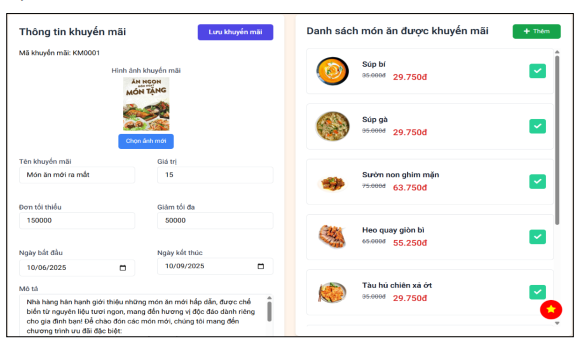
\includegraphics[width=\textwidth]{Chapter_3/Images_c3/khuyenmai.png}
    \caption{Cập nhật chương trình khuyến mãi} 
    \label{fig-logo3}
\end{figure}

%-- Nếu có bảng ---
\begin{table}[H]
\centering
\caption{Kết quả thực nghiệm.}
\begin{tabular}{ccccc}
\toprule
\textbf{STT} & \textbf{Model}   & \textbf{Cột A} & \textbf{Cột B} & \textbf{Cột C} \\ 
\midrule
1 & Thuật toán 1        & 1  & 2  & 3            \\
2 & Thuật toán 2       & 4  & 5  & 6            \\
\bottomrule
\end{tabular}
\label{tab-vidu3}
\end{table}

\subsection{Ưu điểm}

\subsection{Nhược điểm}
